\chapter{Návrh úložiště}
Hlavní motivací pro vytvoření této práce je vytěžování patentů pro účely zjišťování existence napříkad různých technologických vynálezů či algoritmů. Pomocí těchto informací lze zjistit, zda například má smysl vymýšlet nový algoritmus pro určitý problém a neexistuje k němu jiné, lepší řešení, případně vymyslet modifikaci, která zajistí lepší výsledky.
\newline

\noindent Dále je potřebat definovat, co vlastně znamená pojem efektivní vytěžování. Vytěžování lze označit za efektivní, pokud budou splněny tyto podmínky:
\begin{itemize}
\item \textbf{Rychlost} - Vyhledávání musí probíhat v rámci jednotek až desítek sekund (případně jednotky minut, záleží na celkovém počtu patentů a na hardwarové konfiguraci serveru).
\item \textbf{Stabilita} - Server musí být stabilní a nesmí padat při práci s velkým množstvím dat, zvlášť při vyhledávání s použitím složitých dotazů (nařípkad hledání přes více tabulek).
\end{itemize}

\noindent V následujících kapitolách bude popsán postup výběru zdrojů patentů a patentových dat. Následně budou vybrány typy databáze, které budou vhodné pro uložení vybraných patentových dat a následné zvolení existujících řešení.

\section{Výběr patentů}
Při výběru patentů byly stanoveny čtyři podmínky, které museli být splněny:
\begin{itemize}
\item \textbf{Dostupnost} - Patenty musí být dostupné z online stránek / databází bez poplatků.
\item \textbf{Datum} - Patentová přihláška nebo publikace patentu musí být podána alespoň v roce 2000, všechny ostatní patenty budou vyfiltrovány.
\item \textbf{Atributy} - Všechny patenty musí obsahovat povinné atributy (viz kapitola č. \ref{subsec:atributy}).
\item Alternativy jako Užitný a Průmyslový vzor (Návrhový patent) nebudou brány v potaz.
\end{itemize}

\subsection{Zdroje dat}
V dnešním světě existuje několik desítek až stovek patentových zdrojů dat, od webových vyhledávačů v databázi až po plný export databáze s patenty. Velké organizace, jako například \gls{EPO}, \gls{WIPO}, \gls{USPTO}, udržují jedny z největších patentových databází (desítky až stovky milionů patentů), ve kterých lze vyhledávat velké množství informací zdarma za použití webových vyhledávačů na dané stránce organizace. Lze zde najít všechny typy patentů (přihlášky, publikace), národní patenty i patenty registrované například u \gls{EPO}. V případě exportu databází, \gls{USPTO} poskytuje plný export svých databází veřejnosti pro libovolné používání, zcela zdarma. Využití těchto zdrojů dat by bylo určitě skvělé, ale tyto zdroje byly nedávno použity a rozebrány v jiné diplomové práci, proto je vhodné se spíše zaměřit na národní zdroje dat patentů.
\newline
\indent Národní databáze patentů dané země obsahuje všechny národní patenty, některé dokonce i patenty z jiných zemí registrovaných u \gls{EPO}. 
\newline
\indent Při průzkumu bylo zkoumáno celkem 51 národních zdrojů dat (patentových úřadů). V tabulkách č. \ref{tab:table_offices1} a \ref{tab:table_offices2} lze vidět název země, název patentového úřadu v dané zemi, zkratku patentového úřadu (pokud nějakou má) a jestli patentový úřad poskytoval data nebo ne. U každého patentového úřadu byl procházen její oficiální web a zkoumán na dostupnost patentových dat. Většina úřadů má na svých stránkách vyhledávač pro procházení vlastní databáze patentů, ale jen zlomek z nich poskytoval použitelná data zadarmo. Tyto data byla většinou schována pod neodpovídajícím názvem článku / příspěvku, a některé dokonce poskytovaly odkazy ke stažení dat na svých stránkách pouze v národním jazyce (neexistující článek s daty v anglické verzi webu). 
	\begin{table}[H]
	\centering
	\begin{tabular}{|>{\centering\arraybackslash}p{2.2cm}|>{\centering\arraybackslash}p{7.5cm}|>{\centering\arraybackslash}p{2cm}|>{\centering\arraybackslash}p{1cm}|} 
	\hline
	\textbf{Země}    & \textbf{Patentový úřad} & \textbf{Zkratka} & \textbf{Data}                \\ 
	\hline
	Velká Británie & \href{https://www.gov.uk/topic/intellectual-property}{Intellectual Property Office}  & IPO & ANO        \\ 
	\hline
	Arménie & \href{https://www.aipa.am/hy/}{Intellectual Property Office}  & - & NE        \\ 
	\hline
	Austrálie & \href{https://www.ipaustralia.gov.au/}{IP Australia}  & - & ANO         \\ 
	\hline
	Bělorusko & \href{https://www.ncip.by/}{National Center of Intellectual Property}  & NCIP & NE         \\ 
	\hline
	Bulharsko & \href{https://www.bpo.bg/}{Patent Office of Republic of Bulgaria}  & -  & NE       \\ 
	\hline
	Česko & \href{https://upv.gov.cz/}{Industrial Property Office of the Czech Republic}  & -   & ANO      \\ 
	\hline
	Čína & \href{https://www.cnipa.gov.cn/}{China National Intellectual Property Administration}  & CNIPA   & NE      \\ 
	\hline
	Dánsko & \href{https://www.dkpto.org/}{Danish Patent and Trademark Office}  & -    & NE     \\ 
	\hline
	Egypt & \href{http://www.egypo.gov.eg}{Egyptian Patent Office}  & -   & NE      \\ 
	\hline
	Estonsko & \href{https://www.epa.ee/et}{The Estonian Patent Office}  & -   & NE      \\ 
	\hline
	Filipíny & \href{http://www.ipophil.gov.ph/}{Intellectual Property Office of the Philippines}  & IPOPHL & NE        \\ 
	\hline
	Finsko & \href{http://www.prh.fi/en/index.html}{Finnish Patent and Registration Office}  & PRH   & NE      \\ 
	\hline
	Francie & \href{http://www.inpi.fr/}{National Institute of Industrial Property}  & INPI   & ANO      \\ 
	\hline
	Hong Kong & \href{https://www.ipd.gov.hk/index.htm}{Intellectual Property Department}  & -   & NE      \\ 
	\hline
	Chorvatsko & \href{https://www.dziv.hr/}{State Intellectual Property Office of the Republic of Croatia}  & SIPO  & NE       \\ 
	\hline
	Indie & \href{http://www.ipindia.nic.in/}{Office of the Controller General of Patents, Designs and Trade Marks}  & -    & NE    \\ 
	\hline
	Indonésie & \href{http://www.dgip.go.id/}{Directorate General of Intellectual Property}  & DGIP & NE        \\ 
	\hline
	Irsko & \href{https://www.ipoi.gov.ie/en/}{Intellectual Property Office of Ireland}  & IPOI   & NE      \\ 
	\hline
	Island & \href{https://www.isipo.is/}{Icelandic Intellectual Property Office}  & ISIPO    & NE     \\ 
	\hline
	Israel & \href{https://www.gov.il/en/departments/ilpo}{The Israel Patent Office}  & ILPO    & ANO     \\ 
	\hline
	Itálie & \href{https://uibm.mise.gov.it/index.php/it/}{Directorate General for the Protection of Industrial Property}  & -    & ANO*     \\ 
	\hline
	Japonsko & \href{https://www.jpo.go.jp/e/index.html}{Japan Patent Office}  & JPO  & ANO       \\ 
	\hline
	Jižní Korea & \href{http://www.kipo.go.kr/}{Korean Intellectual Property Office}  & KIPO   & ANO      \\ 
	\hline	
	Kanada & \href{https://www.ic.gc.ca/}{Canadian Intellectual Property Office}  & CIPO  & ANO      \\ 
	\hline
	Kuba & \href{http://www.ocpi.cu}{Cuban Industrial Property Office}  & OCPI   & NE      \\ 
	\hline
	Litva & \href{http://vpb.lrv.lt/en/}{State Patent Bureau of the Republic of Lithuania}  & -    & ANO     \\
	\hline
	\end{tabular}
	\caption{Národní patentové úřady a jejich zkratky, část první.}
	\label{tab:table_offices1}
	\end{table}
\newpage
	\begin{table}[H]
	\centering
	\begin{tabular}{|>{\centering\arraybackslash}p{2.2cm}|>{\centering\arraybackslash}p{7.5cm}|>{\centering\arraybackslash}p{2cm}|>{\centering\arraybackslash}p{1cm}|} 
	\hline
	\textbf{Země}    & \textbf{Patentový úřad} & \textbf{Zkratka}        & \textbf{Data}        \\ 
	\hline
 	Lotyšsko & \href{https://www.lrpv.gov.lv/lv}{Patent Office of the Republic of Latvia}  & -    & NE     \\ 
	\hline
	Maďarsko & \href{http://www.hipo.gov.hu/}{Hungarian Intellectual Property Office}  & HIPO   & NE      \\ 
	\hline
	Malajsie & \href{http://www.myipo.gov.my/}{Intellectual Property Corporation of Malaysia}  & MyIPO  & NE       \\ 
	\hline
	Mexiko & \href{https://www.gob.mx/impi/en}{Instituto Mexicano De La Propiedad Industrial}  & IMPI  & ANO       \\ 
	\hline
	Moldova & \href{http://www.agepi.gov.md/}{State Agency on Intellectual Property}  & AGEPI   & NE      \\ 
	\hline
	Německo & \href{http://www.dpma.de/}{German Patent and Trade Mark Office}  & DPMA   & ANO      \\ 
	\hline
	Nizozemsko & \href{http://www.rvo.nl/octrooien}{Netherlands Patent Office}  & -    & NE    \\ 
	\hline
	Norsko & \href{https://www.patentstyret.no/en/}{Norwegian Industrial Property Office}  & NIPO    & NE     \\ 
	\hline
	Nový Zéland & \href{http://www.iponz.govt.nz/}{Intellectual Property Office of New Zealand}  & IPONZ   & ANO      \\ 
	\hline
	Peru & \href{http://www.indecopi.gob.pe/}{National Institute for the Defense of Competition and Protection of Intellectual Property}  & INDECOPI    & ANO     \\ 
	\hline
	Polsko & \href{https://uprp.gov.pl/pl}{Urząd Patentowy Rzeczypospolitej Polskiej}  & UPRP    & ANO     \\ 
	\hline
	Portugalsko & \href{https://inpi.justica.gov.pt/}{Portuguese Institute of Industrial Property}  & -     & ANO    \\ 
	\hline
	Rakousko & \href{http://www.patentamt.at/}{Austrian Patent Office}  & -     & NE    \\ 
	\hline
	Rumunsko & \href{http://www.osim.ro/}{State Office for Inventions and Trademarks}  & OSIM      & NE   \\ 
	\hline
	Rusko & \href{https://rospatent.gov.ru/}{Federal Service for Intellectual Property}  & Rospatent   & ANO      \\ 
	\hline
	Řecko & \href{http://www.obi.gr/el/}{Hellenic Industrial Property Organization}  & HIPO   & NE      \\ 
	\hline
	Singapur & \href{http://www.ipos.gov.sg/}{Intellectual Property Office of Singapore}  & IPOS    & NE     \\ 
	\hline
	Slovensko & \href{https://www.indprop.gov.sk/}{Industrial Property Office of the Slovak Republic}  & -     & NE    \\ 
	\hline
	Slovinsko & \href{http://www.uil-sipo.si/}{Slovenian Intellectual Property Office}  & SIPO   & NE      \\ 
	\hline
	Srbsko & \href{http://www.zis.gov.rs/}{Intellectual Property Office of the Republic of Serbia}  & -   & NE      \\ 
	\hline
	Španělsko & \href{http://www.oepm.es/}{Spanish Patent and Trademark Office}  & OEPM   & ANO      \\ 
	\hline
	Švédsko & \href{http://www.prv.se/}{Swedish Intellectual Property Office}  & PRV   & ANO      \\ 
	\hline
	Švýcarsko & \href{https://www.ige.ch/}{Swiss Federal Institute of Intellectual Property}  & -     & NE    \\ 
	\hline
	Turecko & \href{http://www.turkpatent.gov.tr/}{Turkish Patent and Trademark Office}  & Turkpatent   & NE      \\ 
	\hline
	Ukrajina & \href{https://ukrpatent.org/en}{Ukrainian Intellectual Property Institute}  & Ukrpatent    & NE     \\ 
	\hline
	\end{tabular}
	\caption{Národní patentové úřady a jejich zkratky, část druhá.}
	\label{tab:table_offices2}
	\end{table}
\newpage

\noindent Z celkových 51 patentových zdrojů nám pouze 19 zdrojů poskytuje data. V případě Itálie nám data neposkytuje přímo patentový úřad, ale výzkumný úřad PATIRIS, který poskytuje patentová data z univerzit a veřejných výzkumných ústavů v Itálii. 
\newline
\indent Bohužel ne všechny patentové úřady poskytují svá data zdarma. Celkem tři úřady - Austrálie, Německo, Nový Zéland chtěli za svá data zaplatit. 
\newline
\indent Ještě je potřeba zmínit Japonsko, které svá data poskytuje, ale je potřeba vyplnit formulář, ve kterém bylo potřeba naskenovat oficiální dokument potvrzující adresu školy. Z tohoto důvodu jsme bylo Japonsko jako jako zdroj dat zavrhnuto. Z původních 19 zdrojů dat poskytující data zůstalo nakonec jen 14 zdrojů dat, které poskytují svá data zadarmo.

\subsection{Atributy}\label{subsec:atributy}
Při zadávání práce byly definovány podmínky pro výběr platných zdrojů dat, a jednou z nich bylo i povinnost mít důležité atributy ve struktuře dat patentu. Celkem byly definovány čtyři povinné atributy společně s osmi nepovinnými. Povinné a nepovinné atributy jsou podrobně popsány níže.
\subsubsection{Povinné atributy}
Se zadavatelem bylo domluveno, že validní zdroj patentových dat musí poskytovat patenty obsahující tyto atributy:
\begin{itemize}
\item \textbf{Titulek} - Titulek patentu, který říká o čem daný patent.
\item \textbf{Rok přihlášky / publikace} - Patent musí obsahovat alespoň rok přihlášky / publikace. Publikace / přihláška musí být minimálně z roku 2000, patenty před rokem 2000 budou zamítnuty.
\item \textbf{Autor} - U patentu bude nutné vědět jeho autor (jméno autora, případně název instituce).
\item \textbf{ID patentu} - Patent musí mít nějaké kódové označení / identifikátor, podle kterého ho lze vyhledávat. Identifikátor se bude držet formátu viz obrázek č. \ref{fig:patent_id}, ale nemusí obsahovat všechny položky, protože každá země může některé položky zanedbávat, případně měnit počet znaků v položce, viz tabulka č. \ref{tab:patent_table_id}.
\end{itemize}

	\begin{figure}[H]
	\centering
	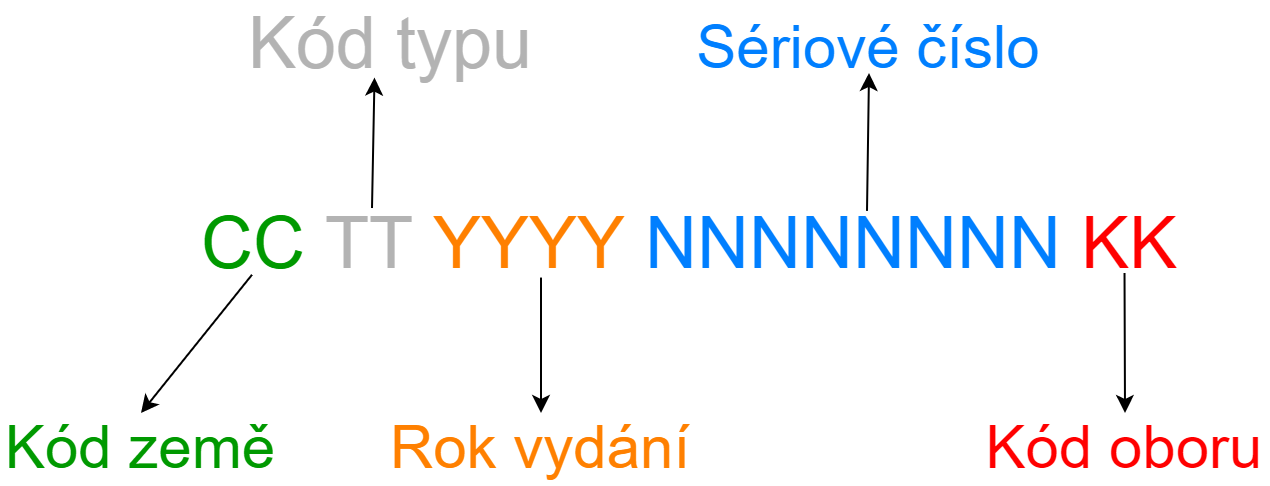
\includegraphics[width=12cm]{img/patent_id}
	\caption{Základní formát pro identifikátor patentu \cite{patent_id_format}.}
	\label{fig:patent_id}
	\end{figure}

	\begin{table}[H]
	\centering
	\begin{tabular}{|>{\centering\arraybackslash}p{2.2cm}|>{\centering\arraybackslash}p{1cm}|>{\centering\arraybackslash}p{2cm}|>{\centering\arraybackslash}p{2cm}|>{\centering\arraybackslash}p{3cm}|>{\centering\arraybackslash}p{1cm}|}
	\hline
	\textbf{Země}    & \textbf{CC} & \textbf{TT} & \textbf{YYYY} & \textbf{NNNNNNNN} & \textbf{KK} \\
	\hline
	Austrálie & AU & & 4 znaky & 6 znaků & ANO \\
	\hline
	Kanada & CA & & & 7 znaků & ANO \\
	\hline
	Čína & CN & 1 znak & & 8 znaků & ANO \\
	\hline
	EPO & EP & & & 7 znaků & ANO \\
	\hline
	Německo & DE & 2 znaky & 4 znaky & 6 znaků & ANO \\
	\hline
	Francie & FR & & & 7 znaků & ANO \\
	\hline
	Velká Británie & GB & & & 7 znaků & ANO \\
	\hline
	Nizozemsko & NL & & & 7 znaků & ANO \\
	\hline
	Japonsko & JP & & 4 znaky & 6 znaků & ANO \\
	\hline
	Korea & KR & 2 znaky & 4 znaky & 7 znaků & ANO \\
	\hline
	Rusko & RU & & 4 znaky & 6 znaků & ANO \\
	\hline
	USA & US & & 4 znaky & 7 znaků & ANO \\
	\hline
	WIPO & PCT & & 4 znaky & 6 znaků & ANO \\
	\hline
	\end{tabular}
	\caption{Aktuálně používané formáty pro patenty z různých zemí \cite{patent_id_format}.}
	\label{tab:patent_table_id}
	\end{table}

\noindent V tabulce č. \ref{tab:table_attributes_critical} lze vidět patenty, poskytované národními patentovými úřady zdarma, obsahují povinné atributy.
	\begin{table}[H]
	\centering
	\begin{tabular}{|>{\centering\arraybackslash}p{2.2cm}|>{\centering\arraybackslash}p{2cm}|>{\centering\arraybackslash}p{3cm}|>{\centering\arraybackslash}p{2cm}|>{\centering\arraybackslash}p{2.5cm}|} 
	\hline
	\textbf{Země}    & \textbf{Titulek patentu} & \textbf{Rok přihlášky / publikace} & \textbf{Autor} & \textbf{ID patentu}                \\ 
	\hline
	Kanada & x & x & x & x \\
	\hline
	Česko & x & x & - & x \\
	\hline
	Litva & x & x & x & x \\
	\hline
	Portugalsko & x & x & x & x \\
	\hline
	Španělsko & x & x & x & x \\
	\hline
	Švédsko & - & x & - & x \\
	\hline
	Izrael & x & x & x & x \\
	\hline
	Itálie & x & x & x & x \\
	\hline
	Mexiko & x & x & x & x \\
	\hline
	Polsko & x & x & - & - \\
	\hline
	Velká Británie & x & x & x & x \\
	\hline
	Rusko & x & x & x & x \\
	\hline
	Peru & x & x & x & x \\
	\hline
	Francie & x & x & x & x \\
	\hline
	\end{tabular}
	\caption{Povinné atributy nacházející se v dostupných patentech.}
	\label{tab:table_attributes_critical}
	\end{table}

\subsubsection{Nepovinné atributy}
Při průzkumu byly zjišťovány i nepovinné atributy, které nemají vliv na výběr zdrojů dat, ale je dobré vědět co který patent z daného patentového zdroje poskytuje za atributy. Nepovinné atributy jsou:
\begin{itemize}
\item \textbf{Abstrakt} - Stručný výtah patentu, který popisuje o čem daný patent je.
\item \textbf{Klíčová slova} - Klíčová sloa nebo fráze spojené s patentem. Mohou sloužit při vyhledávání patentů se stejným zaměřením.
\item \textbf{Reference} - Reference na podobné typy patentů nebo na související patenty (například odkaz na základní verzi algoritmu).
\item \textbf{Žadatel} - Žadatel a autor může být tatáž osoba, ale v některých případech je žadatelem někdo jiný (například autor je zaměstnanec firmy, žadatelem je samotná firma).
\item \textbf{Adresa autora / instituce} - Adresa autora nebo instituce.
\item \textbf{Rodina patentů} - Rodina patentů je kolekce patentových žádostí, které se zaměřují na stejný nebo alespoň podobný technický obsah.
\item \textbf{Obor} - Obor, který daný patent pokrývá.
\item \textbf{Full-text} - Zdroje dat poskytují veškerá data o patentu (nejenom to co je v přihláškách / publikacích, například různé poznámky, obrázky).
\end{itemize}

\noindent V tabulkách č. \ref{tab:table_attributes_notcrit1}, č. \ref{tab:table_attributes_notcrit2} lze vidět patenty, poskytované národními patentovými úřady zdarma, obsahující nepovinné atributy.
	\begin{table}[H]
	\centering
	\begin{tabular}{|c|c|c|c|c|} 
	\hline
	\textbf{Země}    & \textbf{Abstrakt} & \textbf{Klíčová slova} & \textbf{Reference} & \textbf{Žadatel} \\
	\hline
	Kanada & - & - & - & x \\
	\hline
	Česko & x & - & x & - \\
	\hline
	Litva & x & - & - & x \\
	\hline
	Portugalsko & x & - & - & x \\
	\hline
	Španělsko & x & - & - & x \\
	\hline
	Švédsko & x & - & - & - \\
	\hline
	Izrael & - & - & - & x \\
	\hline
	Itálie & - & - & - & x \\
	\hline
	Mexiko & x & - & - & x \\
	\hline
	Polsko & x & x & - & - \\
	\hline
	Velká Británie & - & - & - & - \\
	\hline
	Rusko & - & - & - & - \\
	\hline
	Peru & - & - & - & - \\
	\hline
	Francie & x & - & x & x \\
	\hline
	\end{tabular}
	\caption{Nepovinné atributy nacházející se v dostupných patentech, část první.}
	\label{tab:table_attributes_notcrit1}
	\end{table}

	\begin{table}[H]
	\centering
	\begin{tabular}{|c|c|c|c|c|} 
	\hline
	\textbf{Země}    &  \textbf{Adresa} & \textbf{Rodina patentů} & \textbf{Obor} & \textbf{Full-text} \\
	\hline
	Kanada & x & x & x & - \\
	\hline
	Česko & - & x & x & - \\
	\hline
	Litva & - & x & x & - \\
	\hline
	Portugalsko & - & - & x & - \\
	\hline
	Španělsko & x & - & x & x \\
	\hline
	Švédsko & - & x & x & x \\
	\hline
	Izrael & x & x & - & - \\
	\hline
	Itálie & - & - & - & - \\
	\hline
	Mexiko & - & - & x & - \\
	\hline
	Polsko & - & - & - & - \\
	\hline
	Velká Británie & - & - & x & - \\
	\hline
	Rusko & - & - & - & - \\
	\hline
	Peru & - & - & x & - \\
	\hline
	Francie & - & x & x & - \\
	\hline
	\end{tabular}
	\caption{Nepovinné atributy nacházející se v dostupných patentech, část druhá.}
	\label{tab:table_attributes_notcrit2}
	\end{table}

\subsection{Analýza dat}
Z tabulky č. \ref{tab:table_attributes_critical} lze vidět tři země, jejichž poskytovaná data neobsahují povinné atributy - Česko, Švédsko a Polsko. Pro země, jejichž data obsahující povinné atributy, bude následně provedena hlubší analýza dat - formát dat, počet souborů s daty, struktura dat a počet vyfiltrovaných patentů.

\subsubsection{Velká Británie}
Velká Británie poskytuje svá data v žurnálu ve formátu \gls{XML} nebo \gls{PDF} v týdenních intervalech od roku 2008. Součástí žurnálu jsou záznamy o přihláškách patentů, jejich publikacích, udělených patentech, evropských patentech a patentech, kterým skončila platnost. 
\newline
\indent Celkem bylo staženo 715 žurnálů ve formě \gls{XML} souborů, ze kterých byly použity pouze udělené patenty (granted). Struktura žurnálů zůstává neměnná od roku 2008 až do současnosti. Při filtrování byl nalezen pouze jeden záznam o patentu, který neobsahoval  všechny povinné atributy, z celkového počtu 88 032 patentů.

\subsubsection{Francie}
Francie poskytuje svá data pouze uživatelům, kteří provedli registraci na stránkách francouzské patentové instituce a vyplnili formulář k poskytnutí dat. Data jsou dostupná jak z webové stránky patentové instituce, tak i na \gls{FTP}, ze které si data lze stáhnout. Dostupných typů dat o patentech bylo několik, ale nejdůležitější byly tyto - bibliografická data o patentech a evropské patenty.
\newline
\indent Celkem bylo staženo 2 729 111 souborů s patenty ve formátu \gls{XML}, ze kterých bylo 746 899 unikátních s datem přihlášení od roku 2000. Struktura patentů byla rozdílná jak v rámci typů dat (bibliografické a evropské), tak i v rámci bibliografických dat, kdy struktura patentů v roce 2017 byla jiná než v roce 2021. Bibliografická data obsahovala mnoho duplikátů a patentů, kterým chyběl vždy alespoň jeden povinný atribut (většinou titulek). Většina evropských patentů byla také odfiltrována, stejně jako u bibliografických zde chyběl hlavně titulek. Celkem bylo vyfiltrováno 474 850 patentů.

\subsubsection{Itálie}
Data pro Itálii poskytuje pouze výzkumný úřad PATIRIS, která jsou poskytována jako plný export relační databáze s tabulkama ve formátu \gls{SQL}. Databáze obsahuje celkem 9 tabulek a 21 367 patentů, ze kterých pouze 7 624 obsahuje všechny povinné atributy.

\subsubsection{Izrael}
Izrael poskytuje svá data všem uživatelům v žurnálu ve formátu \gls{XML} v ročních intervalech od roku 2000. Celkem bylo staženo 19 žurnálů, kdy všechny mají stejnou strukturu dat. Žurnál obsahuje údaje jak o publikaci patentu, tak i o jeho žádosti, ale analýza probíhala pouze nad publikacema. Celkem bylo vyfiltrováno 326 patentů kvůli chybějícímu autoru a titulku z celkových 116 380 patentů.

\subsubsection{Kanada}
Kanada poskytuje svá data všem uživatelům ve formátu \gls{XML} v týdenních intervalech od roku 2019. Kanadský patentový úřad poskytuje dva typy patentových dat - bibliografické a full-text.
\newline
\indent Celkem bylo staženo 1 566 425 souborů s patenty, ze kterých bylo 936 464 unikátních s datem přihlášení od roku 2000. Struktura dat se v průběhu let jednou změnila, konkrétně v roce 2022. V bibliografických datech byly údaje pouze pro publikace, zatímco pro full-text se zde nacházel celý popisek patentu i jeho abstrakt. Celkem bylo vyfiltrováno 119 696 patentů kvůli chybějícímu titulku a autorům.

\subsubsection{Litva}
Litva poskytuje svá data všem uživatelům ve formátu \gls{XML} v dvoutýdenních intervalech od konce roku 2021. Patentový úřad v Litvě poskytuje národní i evropské patenty. Celkem bylo staženo 869 souborů s patenty, kde žádnému z nich nechyběl žádný povinný atribut.

\subsubsection{Peru}
Peru poskytuje svá data všem uživatelům ve formátu XLSX. Pouze jeden soubor s daty z roku 2019 byl nalezen na webové stránce patentové instituce v Peru. Soubor obsahuje celkem 23 157 patentů, ze kterých pouze 1 805 je validních, ostatní patenty mají přihlášku před rokem 2000.

\subsubsection{Portugalsko}
Patentová data z Portugalska jsou poskytována na webovém portálu \textit{data.europa.eu}, který spravuje Evropská Unie. Na portále existuje pouze jeden soubor ve formátu \gls{XML}, který obsahuje celkem 69 patentů.

\subsubsection{Rusko}
Rusko poskytuje svá data všem uživatelům ve formátu \gls{CSV} v měsíčních intervalech (od roku 2020) a nepravidelných intervalech (od roku 2017 do roku 2019).
\newline
\indent Celkem bylo staženo 30 souborů, u kterých zůstala struktura dat neměnná. Ve všech souborech existuje celkem 15 920 786 záznamů o patentech, ze kterých pouze 753 970 patentů je unikátních. Celkem bylo vyfiltrováno 139 937 patentů, kde většina z nich měla datum registrace před rokem 2000.

\subsubsection{Španělsko}
Španělsko poskytuje svá data všem uživatelům ve formátu \gls{XML} v denních a měsíčních intervalech od roku 2021, pro data před rokem 2021 existují roční reporty až do roku 1987. Data jsou poskytována ve formě full-textu.
\newline
\indent Celkem bylo staženo 458 566 souborů s patenty, u kterých zůstala struktura dat neměnná po všechny roky (od roku 2004). Z dat bylo odfiltrováno celkem 345 676 patentů, hlavně kvůli chybějícímu autoru.

\subsubsection{Mexiko}
Mexiko poskytuje svá data všem uživatelům ve formátu \gls{XML} v měsíčních intervalech, ale ke stažení jsou pouze data z předcházejícího měsíce. Struktura souborů se za poslední měsíce nezměnila, ale data o patentech obsažená v souborech jsou nevyhovující, protože se zde nachází patentové přihlášky, které jsou zamítnuté, zrušené z důvodu nezaplacení nebo jim vypršela platnost.

\subsection{Závěr průzkumu}
Průzkum národních zdrojů zahrnoval celkem 51 národních patentujících institucí, ze kterých pouze 10 poskytovalo svá data zdarma a splňovala všechny podmínky. V tabulce č. \ref{tab:patent_rozdeleni} lze vidět souhrn výsledků.

	\begin{table}[H]
	\centering
	\begin{tabular}{|>{\centering\arraybackslash}p{3cm}|>{\centering\arraybackslash}p{2cm}|>{\centering\arraybackslash}p{2.2cm}|}
	\hline
	\textbf{Popis}    & \textbf{Počet} & \textbf{Poměr}\\
	\hline
	Nedostupné & 33 & 64,70 \%\\
	\hline
	Nepoužitelné & 4 & 7,85 \%\\
	\hline
	Za peníze & 4 & 7,85 \%\\
	\hline
	Použitelné & 10 & 19,60 \%\\
	\hline
	\end{tabular}
	\caption{Souhrn průzkumu národních patentujících institucí.}
	\label{tab:patent_rozdeleni}
	\end{table}

\noindent Pro všechny použitelné národní zdroje bylo kromě výskytu atributů dále sledováno: formát uložených dat, počet patentů po roce 2000 (včetně roku 2000) obsahující všechny povinné atributy, počet patentů před rokem 2000 a počet duplikátů. Duplikátem se myslí jiná verze daného patentu, protože v průběhu let se mohl měnit obsah patentu a v databázi nechceme ukládat žádné starší verze jednoho patentu (výsledky vyhledávání v databázi nebudou validní). V tabulce č. \ref{tab:final_zdroje} lze vidět všechny validní národní zdroje.
	\begin{table}[H]
	\centering
	\begin{tabular}{|>{\centering\arraybackslash}p{2.2cm}|>{\centering\arraybackslash}p{1.5cm}|>{\centering\arraybackslash}p{3cm}|>{\centering\arraybackslash}p{3cm}|>{\centering\arraybackslash}p{2.2cm}|}
	\hline
	\textbf{Země}    & \textbf{Formát dat} & \textbf{Počet patentů (rok >= 2000)} & \textbf{Počet patentů (rok < 2000)} & \textbf{Počet duplikátů}\\
	\hline
	Velká Británie & XML & 88 032 & 141 & 19\\
	\hline
	Francie & XML & 746 899 & 192 630 & 1 140 084\\
	\hline
	Israel & XML & 116 380 & 0 & 9 956\\
	\hline
	Itálie & SQL & 7 624 & 4 150 & 9 593 \\
	\hline
	Kanada & XML & 936 464 & 130 279 & 499 682\\
	\hline
	Litva & XML & 869 & 0 & 0\\
	\hline
	Peru & XLSX & 1 805  & 21 352 & 0\\
	\hline
	Portugalsko & XML & 69 & 0 & 0\\
	\hline
	Rusko & CSV & 614 256 & 139 714 & 15 166 816\\
	\hline
	Španělsko & XML & 381 713  & 37 612 & 39 241\\
	\hline
	&&&& \\
	\hline
	\textbf{Souhrn} & & \textbf{2 894 111} & \textbf{525 878} & \textbf{16 865 391} \\
	\hline
	\end{tabular}
	\caption{Seznam všech validních národních zdrojů.}
	\label{tab:final_zdroje}
	\end{table}

\noindent V tabulce č. \ref{tab:final_zdroje_filter} lze vidět výsledný počet patentů (po filtraci všech patentů neobsahující povinné atributy - ID, titulek, autor, datum).
	\begin{table}[H]
	\centering
	\begin{tabular}{|>{\centering\arraybackslash}p{2.2cm}|>{\centering\arraybackslash}p{3.5cm}|>{\centering\arraybackslash}p{3cm}|>{\centering\arraybackslash}p{3.5cm}|}
	\hline
	\textbf{Země}  & \textbf{Počet patentů před filtrací} & \textbf{Filtrace} & \textbf{Počet patentů po filtraci} \\
	\hline
	Velká Británie & 88 032 & 1 & 88 031\\
	\hline
	Francie & 746 899 & 474 850 & 272 049\\
	\hline
	Israel & 116 380 & 326 & 116 054 \\
	\hline
	Itálie & 7 624 & 530 & 7 094\\
	\hline
	Kanada & 936 464 & 119 696 & 816 768\\
	\hline
	Litva & 869 & 0 & 869\\
	\hline
	Peru & 1 805  & 0 & 1 805\\
	\hline
	Portugalsko & 69 & 0 & 69\\
	\hline
	Rusko & 614 256 & 223 & 614 033\\
	\hline
	Španělsko & 381 713  & 308 064 & 73 649\\
	\hline
	&&& \\
	\hline
	\textbf{Souhrn} & \textbf{2 894 111} & \textbf{903 690}& \textbf{1 990 421} \\
	\hline
	\end{tabular}
	\caption{Výsledný počet patentů po filtraci.}
	\label{tab:final_zdroje_filter}
	\end{table}

\section{Výběr databáze}
V kapitole č. \ref{chap:databaze} bylo podrobně popsáno co databáze je, jaké typy databází dnes existují (krátký výčet) i nejznámější existující řešení pro popsané typy databází. V této kapitole budou podrobně popsány rozdíly mezi jednotlivými řešeními a následně se vybere nejlepší typ databáze pro ukládání velkého objemu patentových dat. Následně, podle vybraného typu databáze, se vybere nejvhodnější existující řešení.

\subsection{Výběr typu databáze}
Abychom zajistili co nejefektivnější vytěžování, tak je potřeba vybrat co nejvhodnější typ databáze vzhledem k povaze úlohy. V budoucnu se očekává, že počet skladovaných patentů bude v řádech jednotek až desítek milionů (nelze vyvrátit i stovky milionů v případě, že se budou ukládat i patenty z jiných než národních zdrojů).

\subsubsection{Relační databáze}
Relační databáze není vhodným kandidátem pro ukládání nestrukturovaných patentových dat. V databázi sice existuje datový typ \textbf{BLOB}, který umožňuje ukládat binární soubory (v našem případě soubor s patentovými daty), ale nelze to pokládat za nejlepší řešení, když existují například dokumentové databáze. Lze zmínit i datový typ \textbf{TEXT} / \textbf{LONGTEXT}, který umožňuje ukládát velké množství textu a lze ho procházet pomocí full-text vyhledávání, ale výkonnostně a rychlostně se stejně nevyrovná NoSQL databázím. 
\newline
\indent Využití relační databáze by mělo smysl pouze v případě vytváření statistik (například počet v patentů v Kanadě za rok 2020). Tento přístup by ale vyžadoval extrahovat specifická data (například jen povinné atributy) ze souboru pomocí parseru a následné uložení hodnot do tabulek. 

\subsubsection{Objektově-orientovaná databáze}
Objektově-orientovaná databáze, stejně jako relační databáze, není vhodným kandidátem pro ukládání nestrukturovaných dat. Lze argumentovat vytvořením objektů odpovídající struktuře dokumentu, ale při vložení dokumentu s jinou strukturou nastává problém s uložením atributů, které se nenachází v objektu. V některých případech může vysoká složitost systému zpomalovat vyhledávání. Velká výhoda objektově-orientované datábaze spočívá v jednoduchém mapování objektů při práci s objektově-orientovaném programování, které ale v našem případě nemá využití. V případě vytěžování statistik je objektově-orientovaná databáze horší volbou než relační databáze.

\subsubsection{Databáze klíč-hodnota}
Databáze klíč-hodnota je jednoduchá a velice rychlá databáze, která umožňuje ukládat i nestrukturovaná data a nepotřebuje k tomu velké množství paměti. Její nevýhoda je ale v ukládání složitých struktur, které soubory s patenty mají. Lze uložit celou strukturu patentu jako hodnotu, ale následné vyhledávání hodnot pomocí názvů parametrů je nemožné. Použití databáze klíč-hodnota v našem případě není moc vhodné.

\subsubsection{Grafová databáze}
Grafová databáze není vhodným kandidátem pro ukládání patentů, protože se zaměřuje hlavně na vztahy mezi jednotlivými daty, což u patentů nelze a ani není potřeba sledovat.

\subsubsection{Databáze dokumentů}
Databáze dokumentů, jak už název napovídá, je databáze pro efektivní ukládání dokumentů a jejich vytěžování. Umožňuje ukládat velké množství nestrukturovaných dat, její udržba je snadná a akceptuje dokumenty v několika datových formátech. Její velká nevýhoda je v kontrole konzistence, takže se v databázi mohou vyskytovat duplikáty. I přes tuto nevýhodu je dokumentová databáze vhodným kandidátem pro ukládání patentových dat.

\subsubsection{Závěr}
Dokumentová databáze bude použita jako primární databáze, protože umožňuje ukládat nestrukturované dokumenty velice efektivně. Zároveň podporuje vkládání dokumentů ve více formátech, což v případě mnoha národních zdrojů, kdy každý zdroj ukládá dat v jiném formátu, je velice vhodná vlastnost. Její nevýhoda, kontrola konzistence, může být odstraněna pomocí jednoduché aplikace, která bude kontrolovat výskyt patentu v databázi podle jeho identifikátoru (ID). Dokumentová databáze podporuje i full-text vyhledávání pro efektivnější a rychlejší vyhledávání.
\newline
\indent Relační databáze bude použita jako sekundární databáze pro vytěžování, zaměřená hlavně na tvorbu statistik. Relační databáze je vhodnou volbou pro získávání statistik, protože vyhledávání je velice rychlé a snadné. \gls{SQL} dotazy pro statistiky se můžou uložit do pohledů, které zjednoduší uživateli práci se zadáváním dotazů. Lze zmínit i nevýhody jako třeba problém s údržbou nebo potřeba velkého množství paměti. Tyto nevýhody ale nehrají velkou roli v případě jednotek až desítek milionů záznamů.

\subsection{Výběr z existujících řešení}
V dnešní době existuje mnoho dokumentových i relačních databází, placených i zdarma poskytovaných. Placené verze oproti verzím zdarma mají výhodu v lepší podpoře ze strany vývojářů, obsahují více užitečných funkcí a mají lepší zabezpečení. Pro naše účely bohatě postačí verze zdarma.
\newline
\indent Jako existující řešení databáze dokumentů byla vybrána komunitní verze databáze MongoDB. Komunitní verze je zdarma a server lze provozovat jak lokálně, tak i na cloudu, kde MongoDB poskytuje zdarma uložiště o velikosti 512 MB. Pro lepší a spolehlivější vyhledávání v datech bude MongoDB spojena s vyhledávačem Elasticsearch. Elasticsearch je full-textový open-source vyhledávač, který nabízí vysokou dostupnost, rychlost a škálovatelnost. MongoDB sice obsahuje vlastní full-textový vyhledávač, který ale není tak výkonný jako Elasticsearch.
\newline
\indent Jako existující řešení relační databáze byla vybrána komunitní verze databáze MySQL. MySQL je skvělá databáze, která se používá hlavně pro čtení dat. Zároveň je to jedna z nejpoužívanějších relačních databází, což znamená, že je pro ní k dispozici více nástrojů třetích stran.